\documentclass[oneside]{article}
\usepackage[latin1]{inputenc}
\usepackage[brazil]{babel}
\usepackage{graphicx}
\usepackage{listings}
\usepackage{xcolor}
\usepackage{amsmath}
\usepackage{hyperref}
\usepackage{url}
\usepackage{breakurl}
\usepackage[left=2.7cm, right=2.7cm, bottom=3cm]{geometry}
\usepackage{caption}
\usepackage{subcaption}
\usepackage{lipsum}
\usepackage{fancyhdr}
\usepackage{listing}
\usepackage{gensymb}
\usepackage{caption}

%\renewcommand*{\refname}{Refer�ncias Bibliogr�ficas}

\fancyfoot[c]{\thepage}
\fancyhead[ro,le]{}
\fancyhead[lo]{\leftmark}
\fancyhead[re]{\rightmark}

\lstset{%
	linewidth=\textwidth,%framed box is the text size 
	xleftmargin=.25in,
	xrightmargin=.25in, 
	frame=trbl, 
	columns=flexible, 
	captionpos=t, 
	upquote=false,
	basicstyle=\small\ttfamily,
	firstnumber=1,% 
	numberfirstline=false,% 
	numbers=left,%
	numberstyle=\tiny,% 
	stepnumber=5,%
	numbersep=5pt,% 
	backgroundcolor=\color{green!15},% 
	tabsize=4,% 
	keywordstyle=\color{green!65!black},% 
	commentstyle=\color{blue},% 
	stringstyle=\color{magenta},% 
	breaklines=true,% 
	emph={label},%
	abovecaptionskip=10pt,% 
	belowcaptionskip={\abovecaptionskip},%
	showstringspaces=false, 
	literate={�}{{\^{E}}}1
}%

\lstdefinestyle{code} {%
	basicstyle=\ttfamily\footnotesize,
	backgroundcolor=\color{blue!10},
	%escapeinside={@}{@},
	frame=single, 
	captionpos=t,
	upquote=false,
	numberfirstline=false,% 
	stepnumber=5,%
	tabsize=4,% 
	keywordstyle=\color{green!65!black},% 
	commentstyle=\color{blue},%
	stringstyle=\color{magenta},% 
	breaklines=true,% 
	emph={label},%
	abovecaptionskip=10pt,% 
	belowcaptionskip={\abovecaptionskip},%
}%

\title{\huge
	\vspace{40pt}
	Somador Completo de N�meros de 8 bits com Sinal
	\vspace{25pt}
}

\author{
	Cassio Trindade Batista\\
	\texttt{cassio.batista.13@gmail.com}\\
	\texttt{201106840003}
	\and
	Gabriel Peixoto de Carvalho\\
	\texttt{gaburiero.c@gmail.com}\\
	\texttt{201106840010}
	\and
	Pedro Henrique C. F. Soares\\
	\texttt{pedrofigueiredoc@gmail.com}\\
	\texttt{201106840007}
	\and
	Thiago Barros Coelho\\
	\texttt{tbarroscoelho@gmail.com}\\
	\texttt{201106840041}
}
\date{
\vspace{100pt}
\begin{table}[!h]
	\begin{tabular*}{.9\linewidth}{p{.45\linewidth}p{.45\linewidth}}
	& Projeto apresentado � disciplina Projetos de Hardware e Interfaceamento 
	como requisito de avalia��o.
	Professores: Jeferson Breno N. Leite e Adalbery Rodrigues Castro.
	\end{tabular*}
\end{table}
\vfill
Bel�m -- Brasil\\
\vspace{2pt}
Junho/2015
}

\begin{document}
% capa ------------------------------------------------------------------------
\thispagestyle{empty}
\begin{center}

\includegraphics[width=.16\textwidth]{Figures/logo_ufpa}\\

\vspace{12pt}
\bf\large
UNIVERSIDADE FEDERAL DO PAR�\\\vspace{1.5pt}
INSTITUTO DE TECNOLOGIA\\\vspace{1pt}
FACULDADE DE ENGENHARIA DA COMPUTA��O E\\\vspace{1.5pt}
TELECOMUNICA��ES\\

\vspace{120pt}
{\Large
Sistema de Banco de Dados de uma Escola
}

\vfill
\normalsize
Bel�m -- Brasil\\
Junho/2015
\end{center}
%%% EOF %%%u


% T�tulo e Pre�mbulo -----------------------------------------------------------
\newpage
\maketitle
\thispagestyle{empty}

% Sum�rio e Lista de Figuras ---------------------------------------------------
\newpage
\tableofcontents
\listoffigures

% Introdu��o -------------------------------------------------------------------
\newpage
\pagestyle{fancy}
\begin{section}{Enunciado da Quest�o}
\textbf{Para o enunciado abaixo,}\\ 
\textbf{(a) fa�a um modelo conceitual baseado na abordagem Entidade e Relacionamentos
(E-R);  (feito a m�o entregar no dia)... }\\
\textbf{(b) desenhe no dB-designer com todos os campos e gere o esquema do BD (entregar
o esquema textual e diagrama E-R impresso). }\\ 
\textbf{(c) Crie um script para criar o BD no (Interbase ou MySQl...) e um script para
dar carga  com pelo menos 40 alunos/respons�veis 5 professores e duas turmas. E
fa�a todas as consultas em SQL (R1 at� R6), mostrando a sa�da...}\\

Considere uma escola de ensino fundamental. Nesta escola desejam-se informatizar
diversos procedimentos, sendo coletados os requisitos que seguem. Primeiro �
necess�rio um cadastro de pais (ou respons�veis). Cada aluno tem um respons�vel
(um dos pais, ou outra pessoa). Para o respons�vel � necess�rio ter ID, nome e
fone.  Todo respons�vel tem um endere�o (string20 e.g. "rua pio X, nro13").\\
Cada matr�cula de um aluno vale para o ano corrente. Para o aluno guarda-se o
nome e fone. Para cada aluno cria-se um ID (inteiro) que vale para todos os anos
que o aluno permanecer no col�gio. Al�m disso, anualmente, cada aluno recebe um
n�mero de matricula composto por (ano, s�rie, turma, n�mero seq��ncia). Exemplos
de n�meros de matricula 20083TA23, 20061TB05. Numa turma s�o aceitos no m�ximo
50 alunos.\\
S�o registrados os valores das provas bimestrais dos alunos (duas vezes por
semestre), por mat�ria (portugu�s, matem�tica, geografia, etc). Se o aluno tirar
nota inferior a 60 fica em recupera��o no final de cada semestre, recebendo a
nota da recupera��o, que substitui a menor nota dos dois bimestres. Devem ser
mantidos registros de todas as provas e recupera��es todas notas de uma mat�ria
s�o registradas nos campos (B1,B2,B3,B4,R1,R2: numeric(2)) para cada matricula. 
O sistema deve emitir folhas de freq��ncia (Rel 1), com nome do professor de
cada turma e dos alunos, e da identifica��o da sala (ex. S10, S15); emitir 3
relat�rios.  O sistema deve emitir os boletins de notas (Rel 2) bimestrais
(cumulativo para o ano) para cada aluno; emitir relat�rio de notas para 3
alunos; mostram-se as notas das provas, recupera��es e m�dias semestrais e
anuais. O sistema deve emitir um hist�rico cumulativo (Rel 3) para cada aluno
considerando os v�rios anos; emitir 3 hist�ricos. 
Para os professores registram-se � necess�rio ter ID, nome e fone. S�o criados
relat�rios com os totais (quantidade) de alunos de recupera��o de cada turma
(Rel 4), com objetivo de prover orienta��o pedag�gica para os alunos com pais. 
O sistema tamb�m controla o pagamento da mensalidade de cada aluno. S�o emitidos
boletos (Rel 5), com o endere�o do respons�vel; Emitir 2 boletos, com repons�vel
e endere�o e aluno. Para cada aluno devem ser registrados os valores mensais
pagos; s�o registrados para cada ano os valores na base como (valorMens,
m1,m2,m3,m4,...m12:float); meses s�o inicializados zerados, quando pagos
marca-se o valor pago; o vencimento � o dia 7 de cada m�s; � preciso registar a
data do pagto. No momento da matricula � definido o valor a ser pago (valorMens)
que pode ser reajustado durante o ano (somente o valor atual � registrado em
valorMens). A qualquer momento o respons�vel pode solicitar um "extrato" dos
valores pagos e/ou vencidos de um aluno, dentro de um ano (Rel 6); emitir o
comprovante de tr�s alunos. 

\end{section}
%https://en.wikipedia.org/wiki/Turing_machine
%https://pt.wikipedia.org/wiki/Hist�ria_da_computa��o
%%% EOF %%%


% Metodologia: Teorias aplicadas na implementa��o ------------------------------
\begin{section}{Metodologia}
Em eletr�nica, um somador � um circuito digital que, como sugerido pelo pr�prio
nome, efetua a adi��o de n�meros. Na maioria dos computadores, os somadores s�o
utilizados tanto na Unidade L�gica Aritm�tica (ULA) quanto em outras partes do
processador, onde s�o calculados endere�os, �ndices, incremento de operadores,
etc.

\subsection{Meio Somador}
O meio somador soma dois d�gitos bin�rios de um bit cada. A
Figura~\ref{fig:halfadder} mostra o esquem�tico do sistema, o qual possui uma
porta l�gica do tipo \texttt{XOR} e uma do tipo \texttt{AND}; duas entradas, $A$
e $B$, que representam os bits a serem somados; a sa�da $S$, resultado da
soma; e a sa�da $C$, que � o bit de \textit{carry} ou ``vai um'', 
que nada mais � que um bit de \textit{overflow}.

\begin{figure}[!h]
	\centering
	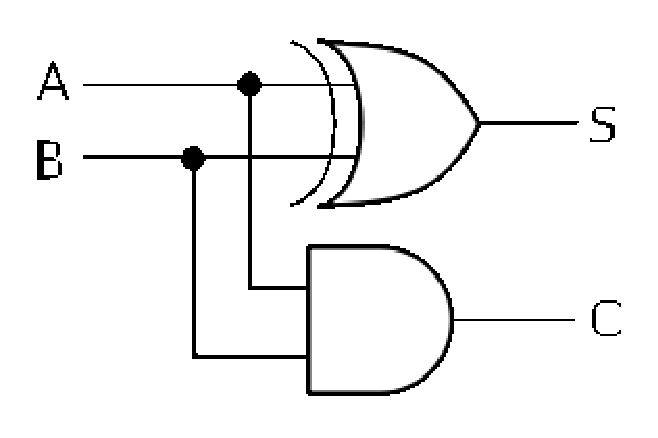
\includegraphics[width=.30\textwidth]{Figures/halfadder}
	\caption{Esquem�tico de um meio somador.}
	\label{fig:halfadder}
\end{figure}

As sa�das do esquem�tico podem ser escritas em fun��o das entradas com aux�lio
da �lgebra de Boole, como mostrado abaixo:
\begin{gather*}
	S = A \oplus B \\
	C = A \ \& \ B \notag
\end{gather*}

A Tabela~\ref{tab:halfadder} mostra a tabela verdade do circuito, bem como sua
representa��o em decimal.
\begin{table}[!h]
\centering
\caption{Tabela verdade de um meio somador.}
\label{tab:halfadder}
\begin{tabular}{cc|cc|c}
	\hline
	$A$ & $B$ & $C$ & $S$ & Decimal \\
	\hline
	0 & 0 & 0 & 0 & 0: 0+0=00\\
	0 & 1 & 0 & 1 & 1: 0+1=01\\
	1 & 0 & 0 & 1 & 1: 1+0=01\\
	1 & 1 & 1 & 0 & 2: 1+1=10\\
	\hline
\end{tabular}
\end{table}

\subsection{Somador Completo}
Um somador completo de um bit adiciona os bits colocados em suas tr�s entradas,
geralmente representadas como $A$, $B$ e $C_{in}$, sendo as duas primeiras as
parcelas e a �ltima, um bit oriundo da soma anterior. O circuito produz duas
sa�das, o resultado $S$ da soma e o bit de \textit{carry} $C_{out}$, o qual
servir� como entrada para uma eventual pr�xima soma.
A Figura~\ref{fig:fulladder} ilustra o esquem�tico de um somador completo.
Nota-se facilmente que o circuito � constru�do por um arranjo de dois meio
somadores, com duas portas do tipo \texttt{XOR}, duas do tipo \texttt{AND} e uma
do tipo \texttt{OR}.

\begin{figure}[!h]
	\centering
	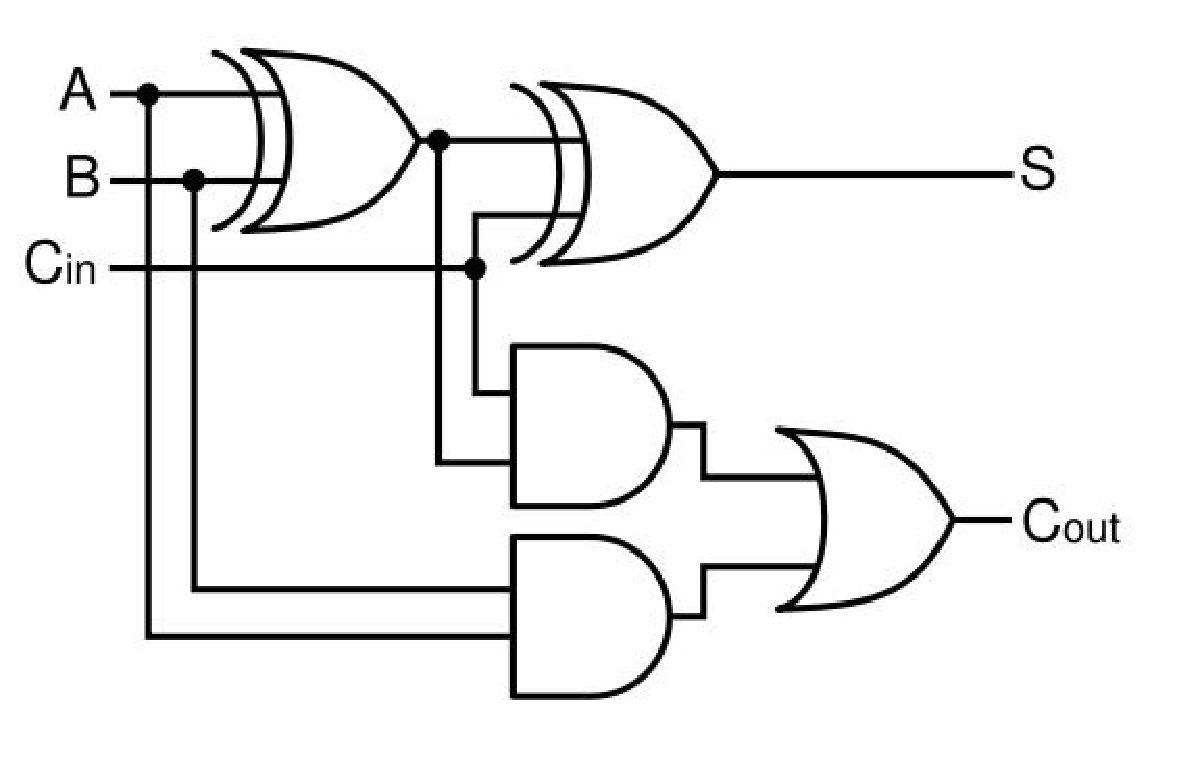
\includegraphics[width=.40\textwidth]{Figures/fulladder}
	\caption{Esquem�tico de um somador completo de 1 bit.}
	\label{fig:fulladder}
\end{figure}

As sa�das podem ser escritas do esquem�tico podem ser escritas em fun��o das
entradas de acordo com a �lgebra de Boole, como mostrado abaixo:
\begin{gather*}
	S = A \oplus B \oplus C_{in} \\
	C_{out} = (A \ \& \ B) + ((A \oplus B) \ \& \ C_{in}) \notag
\end{gather*}

\begin{table}[!h]
\centering
\caption{Tabela verdade de um somador completo.}
\label{tab:fulladder}
\begin{tabular}{ccc|cc|c}
	\hline
	$A$ & $B$ & $C_{in}$ & $C_{out}$ & $S$ & Decimal \\
	\hline
	0 & 0 & 0 & 0 & 0 & 0: 0+0+0=00 \\
	0 & 1 & 0 & 0 & 1 & 1: 0+1+0=01 \\
	1 & 0 & 0 & 0 & 1 & 1: 1+0+0=01 \\
	1 & 1 & 0 & 1 & 0 & 2: 1+1+0=10 \\
	0 & 0 & 1 & 0 & 1 & 1: 0+0+1=01 \\
	0 & 1 & 1 & 1 & 0 & 2: 0+1+1=10 \\
	1 & 0 & 1 & 1 & 0 & 2: 1+0+1=10 \\
	1 & 1 & 1 & 1 & 1 & 3: 1+1+1=11 \\
	\hline
\end{tabular}
\end{table}

O modelo abaixo mostra como ocorre a adi��o de dois n�meros de 8 bits cada. 
Come�ando da direita para a esquerda, deve-se sempre representar o resultado da
soma com dois bits, sendo o mais significativo ``carregado'' para a pr�xima
soma. Tal MSB � mostrado na parte de superior do primeiro vetor de bits e 
representa o bit de \textit{carry}; analogamente, o LSB representa o resultado
apresentado na sa�da $S$. A l�gica da soma segue a tabela verdade mostrada na
Tabela~\ref{tab:fulladder}.

\begin{table}[!h]
\centering
\begin{tabular}{llllllllll}
	${}^1$  & $1^1$ & $1^0$ & $0^1$ & $0^1$ & $1^1$ & $1^0$ & $1^0$ & $0^x$ & +\\
			& $0  $ & $1  $ & $0  $ & $1  $ & $1  $ & $1  $ & $0  $ & $0  $ &  \\
	\hline
		$1$ & $0  $ & $0  $ & $1  $ & $0  $ & $1  $ & $0  $ & $1  $ & $0  $ \\
\end{tabular}
\end{table}

A Figura~\ref{fig:fulladder4} mostra um somador completo de 4 bits. Nota-se que,
para somar dois n�meros de $n$ bits, ser� necess�rio um arranjo de $n$ somadores
completos, onde o \textit{carry} de sa�da $C_{out}$ do LSB vai sendo 
sucessivamente ``carregado'' at� que se chegue ao bloco somador referente ao MSB
do resultado $S$. Para melhor entendimento, denota-se $S_4$ como o MSB e $S_1$
como o LSB. O �ltimo $C_{out}$, mostrado mais � direita, define o sinal do
resultado: ``1'' representa negativo e ``0'', positivo.

\begin{figure}[!h]
	\centering
	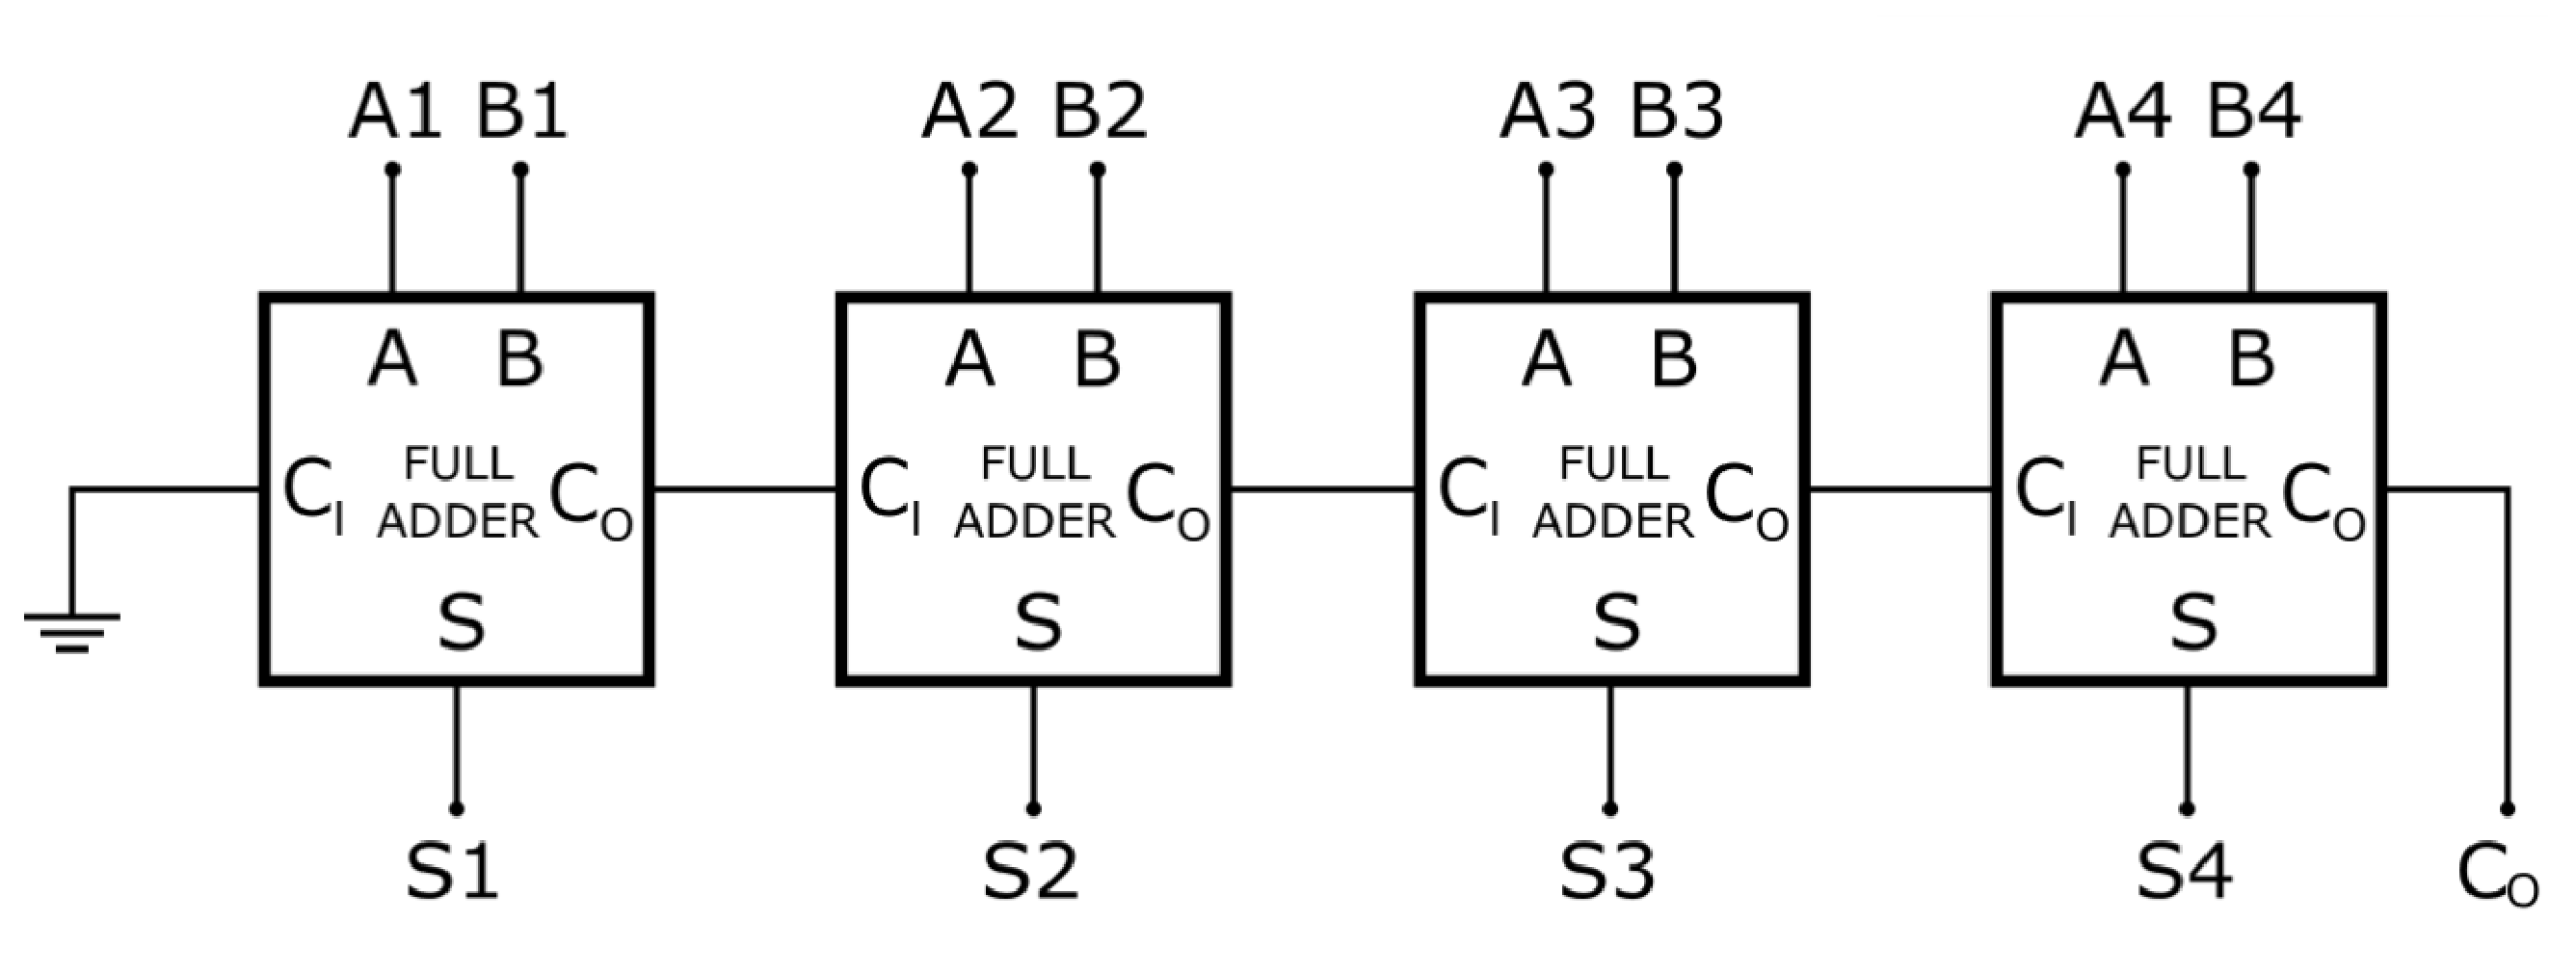
\includegraphics[width=.65\textwidth]{Figures/fulladder4}
	\caption{Esquem�tico de um somador completo de 4 bits.}
	\label{fig:fulladder4}
\end{figure}

\subsection{Complemento de dois}
O somador completo descrito acima t�m sua funcionalidade bem definida ao somar
um par de bits com um bit de \textit{carry} da opera��o anterior. Entretanto,
� v�lido se perguntar: como o resultado consegue ser apresentado de forma
correta na sa�da sem que o bloco fa�a distin��o entre decimais positivos ou
negativos? A explica��o est� na forma em como os bits s�o representados
dependendo do seu sinal.

O complemento de dois, tamb�m conhecido como complemento para dois ou
complemento a dois, � um tipo de representa��o bin�ria de n�meros com sinal
amplamente usada nas arquiteturas dos dispositivos computacionais modernos. O
modelo, mostrado na Figura~\ref{fig:complement2}, revela que o MSB do n�mero
bin�rio define o sinal: se for ``1'', o n�mero � negativo; se for ``0'', �
positivo. Portanto, no caso da aplica��o de um somador de 8 bits, restam apenas
7 bits para representar o m�dulo ou valor real do n�mero, os quais definem uma
precis�o de $-128_{10}$ � $+127_{10}$.

\begin{figure}[!h]
	\centering
	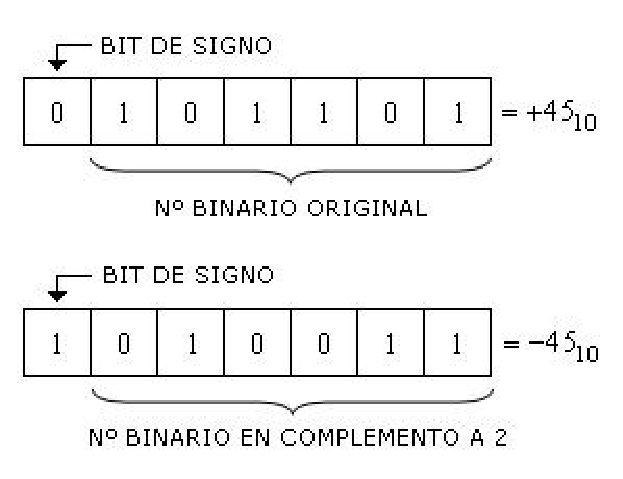
\includegraphics[width=.33\textwidth]{Figures/complement2}
	\caption{Exemplo da representa��o bin�ria positiva e negativa do n�mero decimal ``45''.}
	\label{fig:complement2}
\end{figure}

Para calcular o complemento de dois de um n�mero, o primeiro passo � fazer o 
complemento de um e, ap�s inverter-se todos os bits, soma-se um ao resultado
parcial.

\subsection{Codifica��o Bin�ria Decimal}
A codifica��o bin�ria decimal � importante para podermos converter a sa�da dos
somadores para n�meros decimais e assim poder mostr�-los no display de 7
segmentos. A codifica��o � realizada atrav�s de um algoritmo chamado
\emph{doubledabble}, exemplificado na \ref{fig:bcd}.

\begin{figure}[!h]
	\centering
	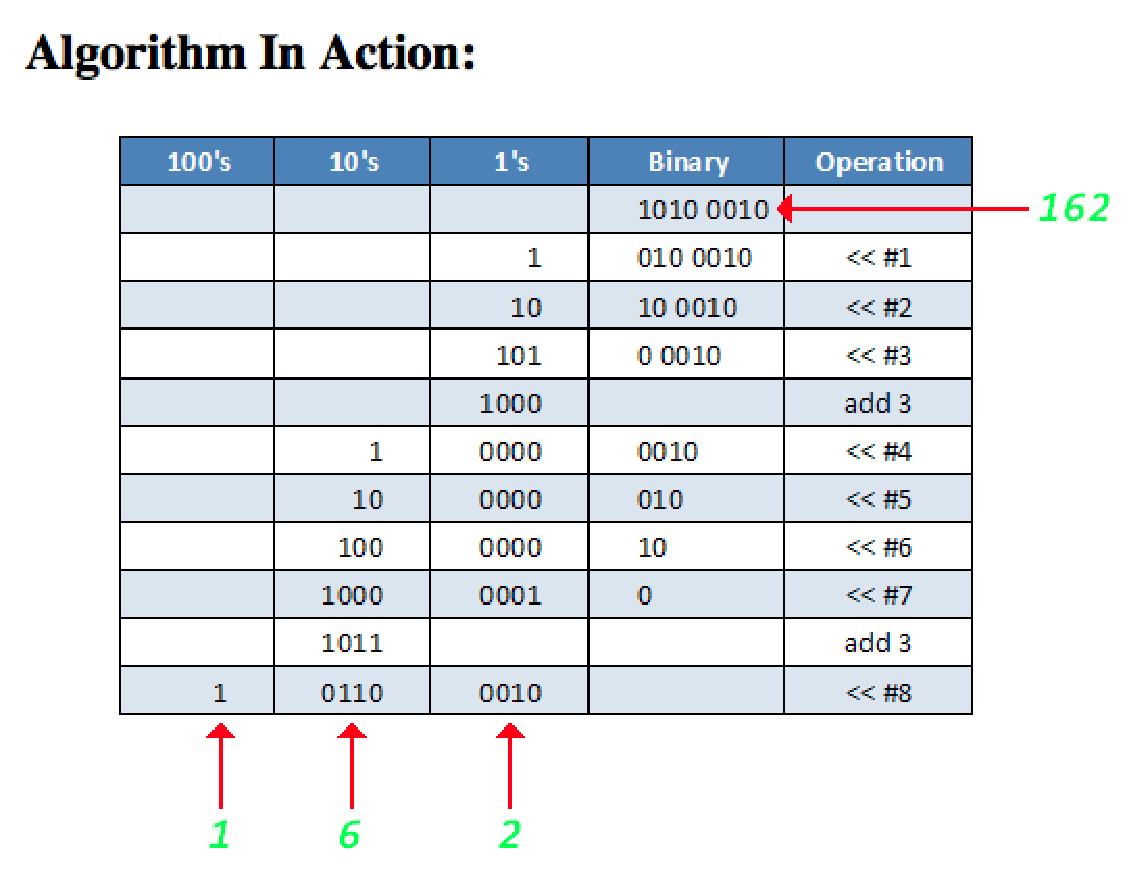
\includegraphics[width=.33\textwidth]{Figures/bcd_exp}
	\caption{Exemplo da convers�o bin�rio para BCD}
	\label{fig:bcd}
\end{figure}


\end{section}
%%% EOF %%%


% Implementa��o: Funcionamento do circuito -------------------------------------
\begin{section}{Implementa��o}
A  implementa��o do scripts foi realizada no software
\textbf{mysql-workbench} usando \textbf{localhost@root} como servidor.\\
As consultas foram feitas seguindo o que era requerido no enunciado da quest�o.

\lstinputlisting[language=SQL]{../db_designer/consultas_r1_r6.sql}

\end{section}
%%% EOF %%%


% An�lise e Simula��o: Modelsim ------------------------------------------------
\begin{section}{Resultados}

\subsection{Diagrama do Sistema}

\begin{figure}
    \centering
    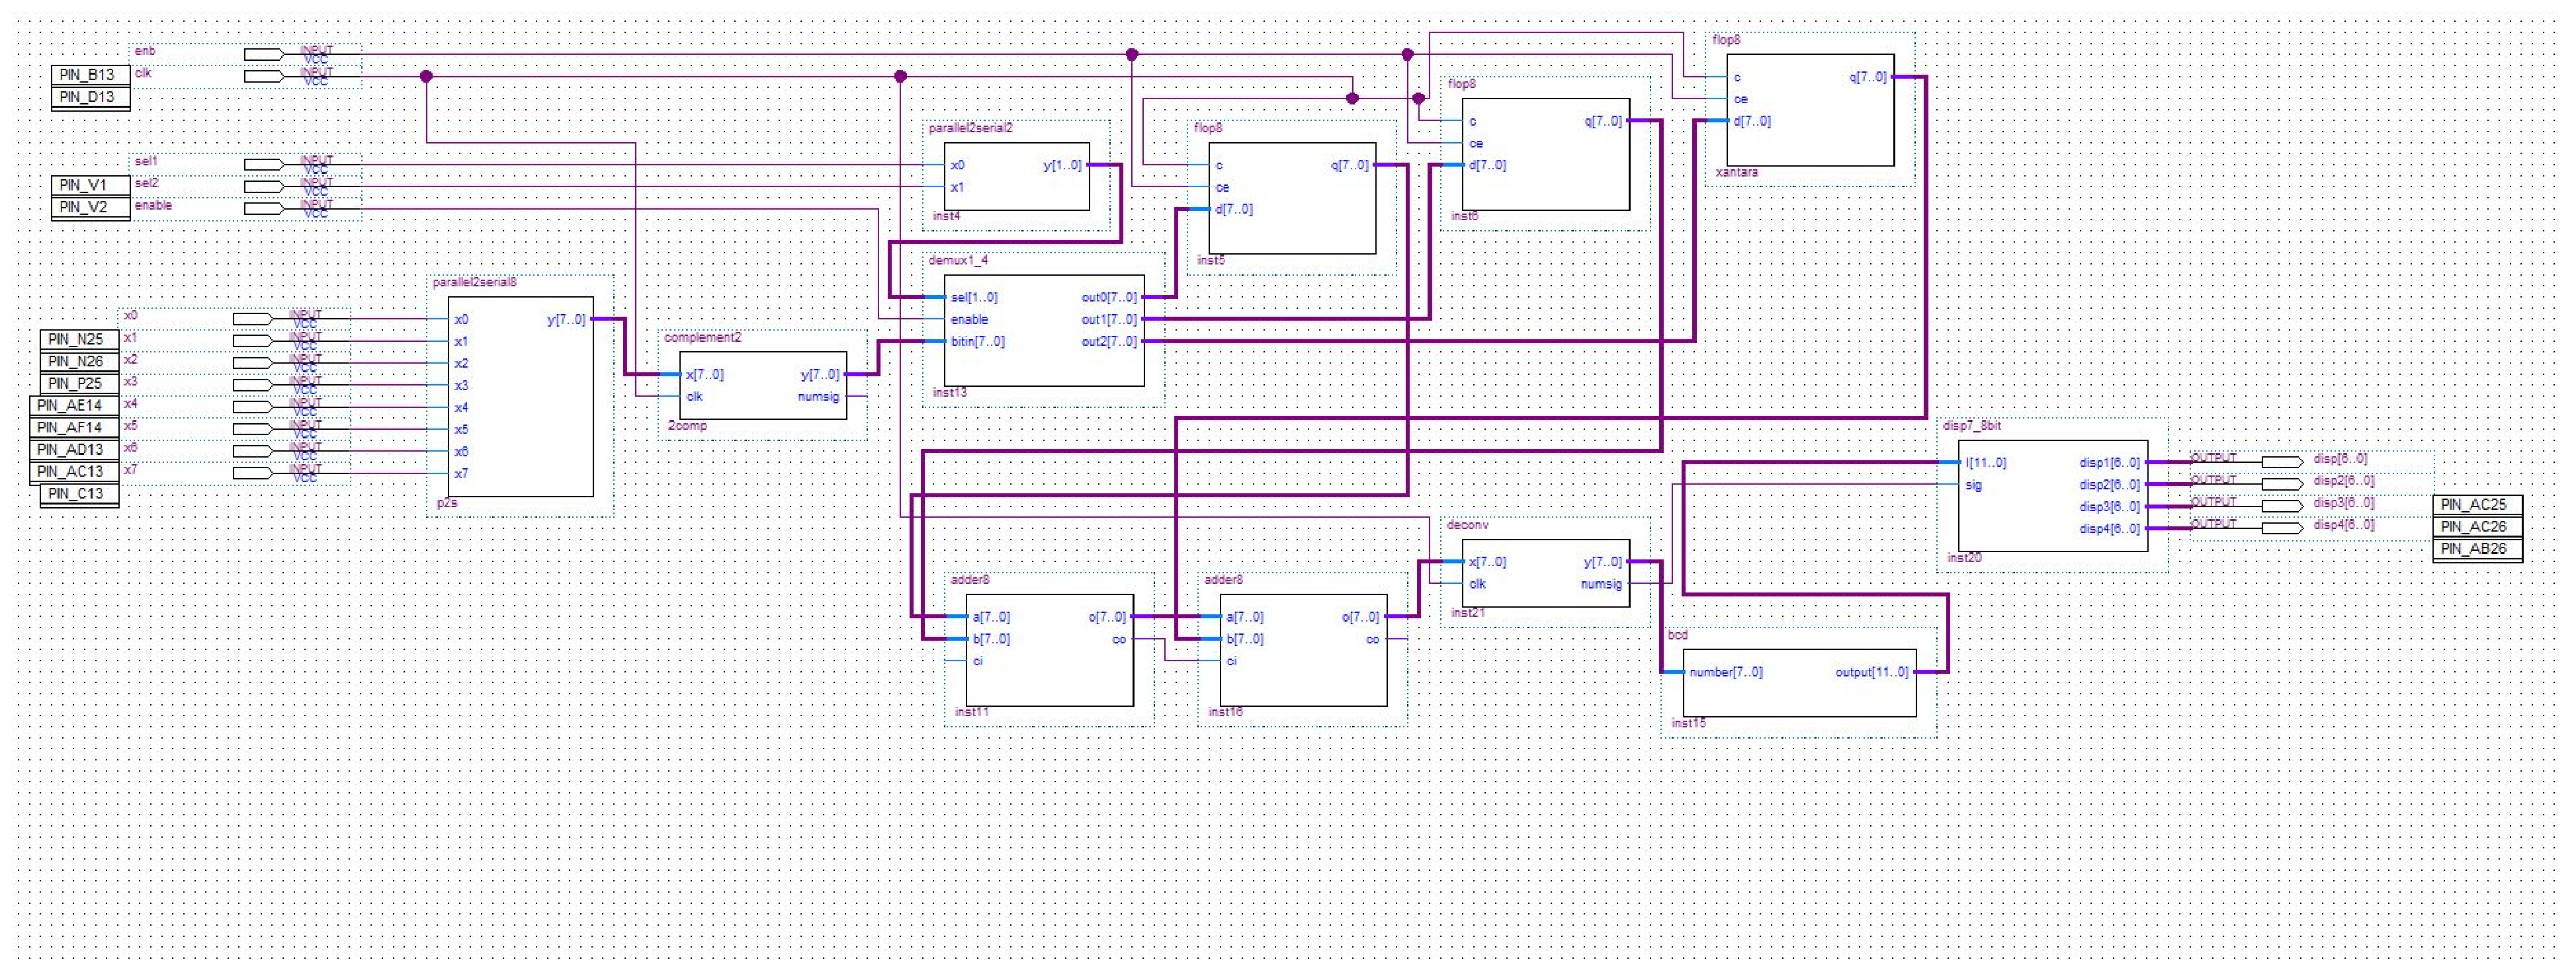
\includegraphics[width=.90\textwidth]{Figures/system_sch}
    \caption{Esquem�tico do Sistema no QuartusII}
    \label{fig:system}
\end{figure}

\subsection{Simula��o}
Todos os blocos do sistema foram devidamente simaulado sno \emph{ModelSim},
muitos por se tratarem de blocos intermedi�rios no sistema, n�o havia muito
sentido em algumas delas.\\
Abaixo � mostrada a sa�da da simula��o do bloco somador:

\begin{figure}
    \centering
    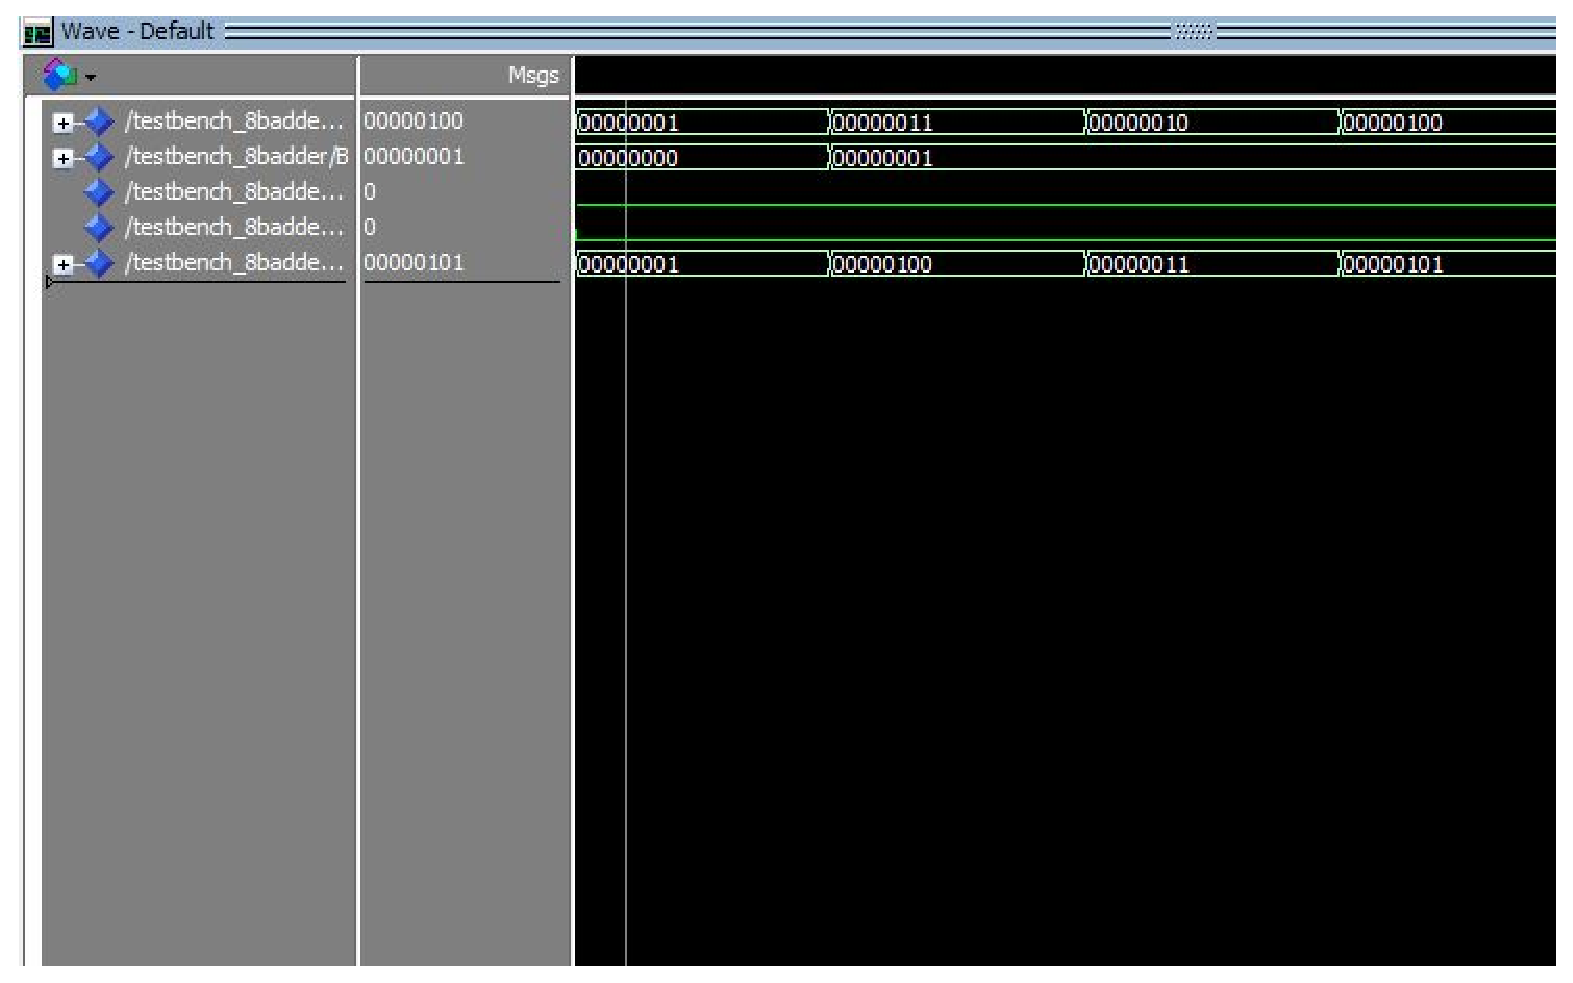
\includegraphics[width=.85\textwidth]{Figures/tb_adder8}
    \caption{Esquem�tico do Sistema no QuartusII}
    \label{fig:system}
\end{figure}

\subsection{Execu��o}
Na finaliza��o do projeto h� alguns pontos a serem salientados.\\

\begin{itemize}
    \item Durante o desenvolvimento do sistema houveram algumas diferen�as na simula��o e
no c�digo que foi mebarcado na fpga, ent�o a partir de certo ponto foi optado o
teste somente na placa.
    \item N�o houve tempo para tratamento de estouro de buffer, ent�o em alguns
        casos a sa�da era o resultado somado com um, o que foi resolvido
        retirando a liga��o entre carry in/carry out do primeiro para o segundo
        somador.
\end{itemize}

\end{section}
%%% EOF %%%


\bibliographystyle{ieeetr}
\bibliography{tech_report}

% C�digos e Background Matem�tico ----------------------------------------------
\newpage
\appendix
%\input{apendice}
\end{document}
%%% EOF %%%
